%%%%%%%%%%%%%%%%%%%%%%%%%%%%%%%%%%%%%%%%%
% Beamer Presentation
% LaTeX Template
% Version 2.0 (27/IX/15)
%
% This template has been downloaded from http://www.LaTeXTemplates.com
% and modified by Semen Martynov <semen.martynov@gmail.com>
%
% License:
% CC BY-NC-SA 3.0 (http://creativecommons.org/licenses/by-nc-sa/3.0/)
%
%%%%%%%%%%%%%%%%%%%%%%%%%%%%%%%%%%%%%%%%%

%----------------------------------------------------------------------------------------
%	PACKAGES AND THEMES
%----------------------------------------------------------------------------------------

\documentclass{beamer}

\mode<presentation> {

% The Beamer class comes with a number of default slide themes
% which change the colors and layouts of slides. Below this is a list
% of all the themes, uncomment each in turn to see what they look like.

%\usetheme{default}
%\usetheme{AnnArbor}
%\usetheme{Antibes}
%\usetheme{Bergen}
%\usetheme{Berkeley}
%\usetheme{Berlin}
%\usetheme{Boadilla}
%\usetheme{CambridgeUS}
%\usetheme{Copenhagen}
%\usetheme{Darmstadt}
%\usetheme{Dresden}
%\usetheme{Frankfurt}
%\usetheme{Goettingen}
%\usetheme{Hannover}
%\usetheme{Ilmenau}
%\usetheme{JuanLesPins}
%\usetheme{Luebeck}
\usetheme{Madrid}
%\usetheme{Malmoe}
%\usetheme{Marburg}
%\usetheme{Montpellier}
%\usetheme{PaloAlto}
%\usetheme{Pittsburgh}
%\usetheme{Rochester}
%\usetheme{Singapore}
%\usetheme{Szeged}
%\usetheme{Warsaw}

% As well as themes, the Beamer class has a number of color themes
% for any slide theme. Uncomment each of these in turn to see how it
% changes the colors of your current slide theme.

%\usecolortheme{albatross}
%\usecolortheme{beaver}
%\usecolortheme{beetle}
%\usecolortheme{crane}
%\usecolortheme{dolphin}
%\usecolortheme{dove}
%\usecolortheme{fly}
%\usecolortheme{lily}
%\usecolortheme{orchid}
%\usecolortheme{rose}
%\usecolortheme{seagull}
%\usecolortheme{seahorse}
%\usecolortheme{whale}
%\usecolortheme{wolverine}

%\setbeamertemplate{footline} % To remove the footer line in all slides uncomment this line
%\setbeamertemplate{footline}[page number] % To replace the footer line in all slides with a simple slide count uncomment this line

%\setbeamertemplate{navigation symbols}{} % To remove the navigation symbols from the bottom of all slides uncomment this line
\setbeamertemplate{caption}[numbered] % Image numbers
}

%%%% Charset (don't forget about texlive-lang-cyrillic)
\usepackage{cmap}							% make PDF files searchable and copyable
\usepackage[utf8x]{inputenc}				% accept different input encodings
\usepackage[T2A]{fontenc}					% russian font
\usepackage[russian]{babel}					% multilingual support (T2A)

%%%% Graphics
%\usepackage[dvipsnames]{xcolor}			% driver-independent color extensions
\usepackage{graphicx}						% enhanced support for graphics
\usepackage{wrapfig}						% produces figures which text can flow around

%%%% Math
\usepackage{amsmath}						% American Mathematical Society (AMS) math facilities
\usepackage{amsfonts}						% fonts from the AMS
\usepackage{amssymb}						% additional math symbols

%%%% Typograpy (don't forget about cm-super)
\usepackage{microtype}						% subliminal refinements towards typographical perfection
%\linespread{1.3}							% line spacing
\setlength{\parindent}{0pt}					% we don't want any paragraph indentation
\usepackage{parskip}						% some distance between paragraphs

%%%% Tables
\usepackage{booktabs}						% Allows the use of \toprule, \midrule and \bottomrule in tables
%\usepackage{tabularx}						% tables with variable width columns
%\usepackage{multirow}						% for tabularx
%\usepackage{hhline}							% for tabularx

%%%% Graph
%\usepackage{tikz}							% package for creating graphics programmatically
%\usetikzlibrary{arrows}						% edges for tikz

%%%% Other
%\usepackage{url}							% verbatim with URL-sensitive line breaks
%\usepackage{fancyvrb}						% sophisticated verbatim text (with box)

\makeatletter
\def\verbatim{\tiny\@verbatim \frenchspacing\@vobeyspaces \@xverbatim}
\makeatother

%----------------------------------------------------------------------------------------
%	TITLE PAGE
%----------------------------------------------------------------------------------------

\title[Кэш-независимые алгоритмы]{Кэш-независимые алгоритмы:\\анализ алгоритма перемножения квадратных матриц} % The short title appears at the bottom of every slide, the full title is only on the title page

\author{Чёрная команда} % Your name
\institute[СПбПУ] % Your institution as it will appear on the bottom of every slide, may be shorthand to save space
{
Санкт-Петербургский политехнический университет Петра Великого \\ % Your institution for the title page
\medskip
\textit{Антон Абрамов <abramov91@mail.ru>\\
Владислав Бусаров <happyfanik@yandex.ru>\\
Сергей Дедков <dsv.mail@yandex.ru>\\
Семён Мартынов <semen.martynov@gmail.com>\\
Николай Патраков <noon.vlg@gmail.com>} % Your email address
}
\date{\today} % Date, can be changed to a custom date

\begin{document}

\begin{frame}
\titlepage % Print the title page as the first slide
\end{frame}

\begin{frame}
\frametitle{Содержание} % Table of contents slide, comment this block out to remove it
\tableofcontents % Throughout your presentation, if you choose to use \section{} and \subsection{} commands, these will automatically be printed on this slide as an overview of your presentation
\end{frame}

%----------------------------------------------------------------------------------------
%	PRESENTATION SLIDES
%----------------------------------------------------------------------------------------

%------------------------------------------------
\section{Введение}
%------------------------------------------------

\begin{frame}
\frametitle{Введение}

\begin{block}{Кэш-зависимымые алгоритмы (англ. cache-conscious)}
При разработке учитываются конкретные характеристики кэша на целевой машине, такие как ассоциативность или размер кэш-блока.
\end{block}
\bigskip

\begin{block}{Кэш-независимые алгоритмы (англ. cache-oblivious)}
При разработке не делается предположений о реальной структуре кэша (а реальная производительность не должна заметно деградировать), но используется модель "идеального кэша".
\end{block}

\end{frame}

%------------------------------------------------

\begin{frame}
\frametitle{Введение: разделяй-и-властвуй}

Исторически лучшую производительность показывали кэш-зависимые алгоритмы, однако имеется предположение, что кэш-независимые алгоритмы так же эффективны как и кэш-зависимые алгоритмы при использовании определённых методик, таких как подход разделяй-и-властвуй (divide-and-conquer).\\~\\

Поскольку алгоритм рекурсивно разбивает подзадачи на более мелкие куски, то в какой-то момент, подзадача станет умещаться в кэш, а последующее разбиение обеспечивает умещение подзадачи в
кэш-строку.Соответственно прекращаются кэш-промахи для более мелких подзадач.
\end{frame}

%------------------------------------------------
\section{Идеальный кэш}
%------------------------------------------------

\begin{frame}
\frametitle{Идеальный кэш}

\begin{figure}
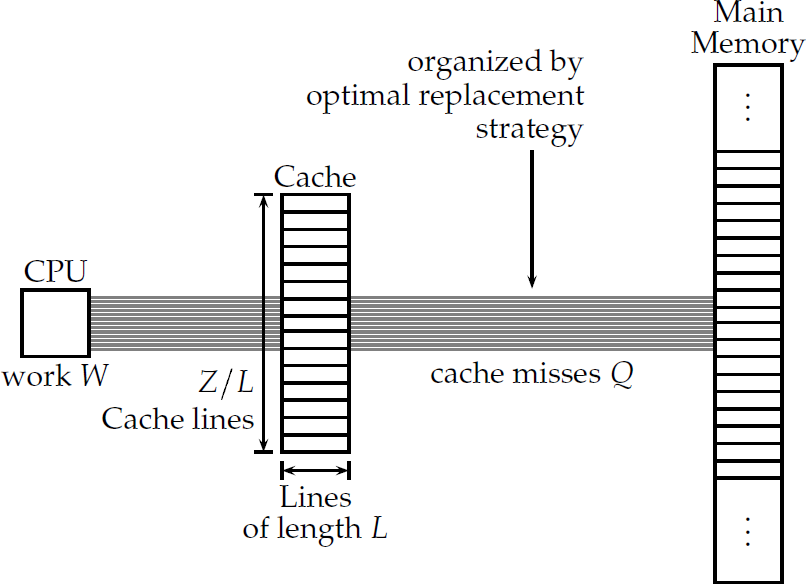
\includegraphics[scale=0.35]{res/pic001}
\caption{Модель идеального кэша}
\end{figure}

\end{frame}
%------------------------------------------------

\begin{frame}
\frametitle{Идеальный кэш: допущения}
Следующие четыре допущения являются ключевыми в модели идеального кэша:\\~\\

\begin{enumerate}
\item \textbf{Оптимальный алгоритм замены}: алгоритм выбора блока кэша, который заменяется при кэш-промахе, когда кэш заполнен. Мы используем LRU (Least Recently Used)
\item \textbf{Два уровня памяти}: должны удовлетворять свойству включения (данные не могут находиться на уровне $i$, если они не представлены на уровне памяти $i + 1$), а размер $i$-го уровня памяти, строго меньше размера $i + 1$ уровня.
\item \textbf{Полная ассоциативность}: если строка была подгружена в кэш из основной памяти, то она может оказать в любой части кэша.
\item \textbf{Автоматическая замена}: Когда необходимо подгрузить данные из основной памяти, это происходит автоматически средствами операционной системы или аппаратуры, но не алгоритма.
\end{enumerate}
\end{frame}

%------------------------------------------------
\section{Алгоритмы}
%------------------------------------------------

%------------------------------------------------
\subsection{Последовательный алгоритм}
%------------------------------------------------

\begin{frame}
\frametitle{Последовательный алгоритм}

Алгоритм является итеративным и ориентирован на последовательное вычисление строк матрицы С.

\begin{figure}
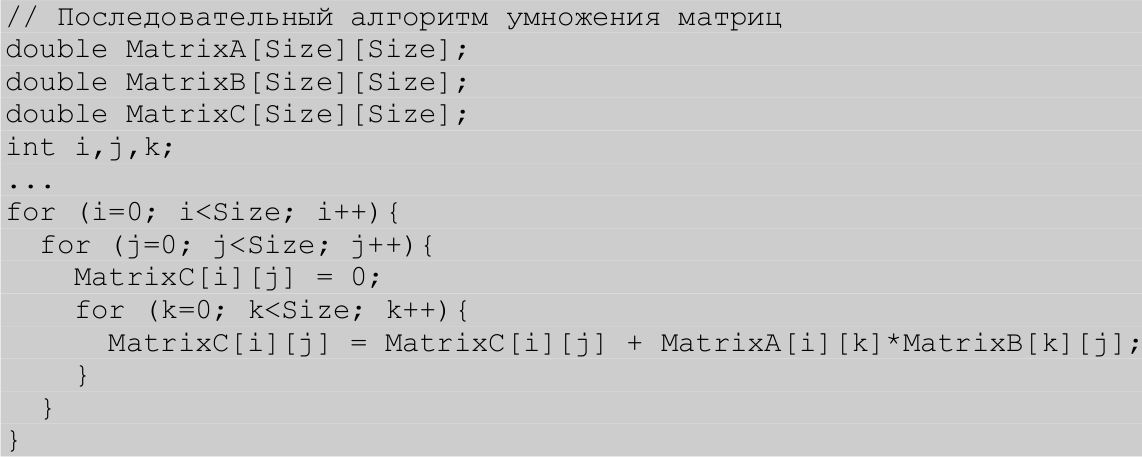
\includegraphics[scale=0.30]{res/pic002}
\caption{Последовательный алгоритм умножения двух квадратных матриц}
\end{figure}

\end{frame}

%------------------------------------------------

\begin{frame}
\frametitle{Последовательный алгоритм}

\begin{figure}
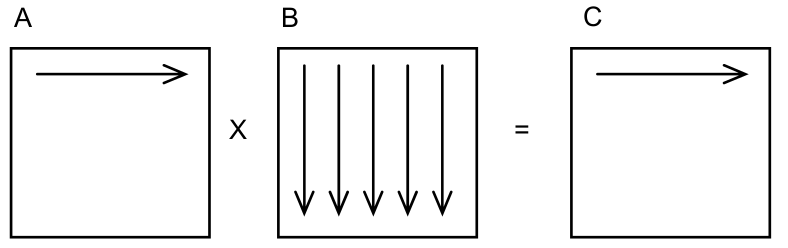
\includegraphics[scale=0.30]{res/pic003}
\caption{При итерации по $i$ используется строка матрицы A и все столбцы матрицы B. Построчное хранение данных многомерных массивов в языке С, приводит к промахам при обращении столбцам!}
\end{figure}

Поскольку каждый элемент результирующей матрицы есть скалярное произведение строки и столбца исходных матриц, то для вычисления всех элементов матрицы С размером n×n необходимо выполнить $n^2 \times ( 2n - 1 )$ скалярных операций и затратить время
\begin{center}
 $T_11 = n^2 \times ( 2 n − 1 ) \times \tau$\\
(где $\tau$ время выполнения одной скалярной операции)
\end{center}

\end{frame}

%------------------------------------------------

\begin{frame}
\frametitle{Последовательный алгоритм}

\begin{figure}
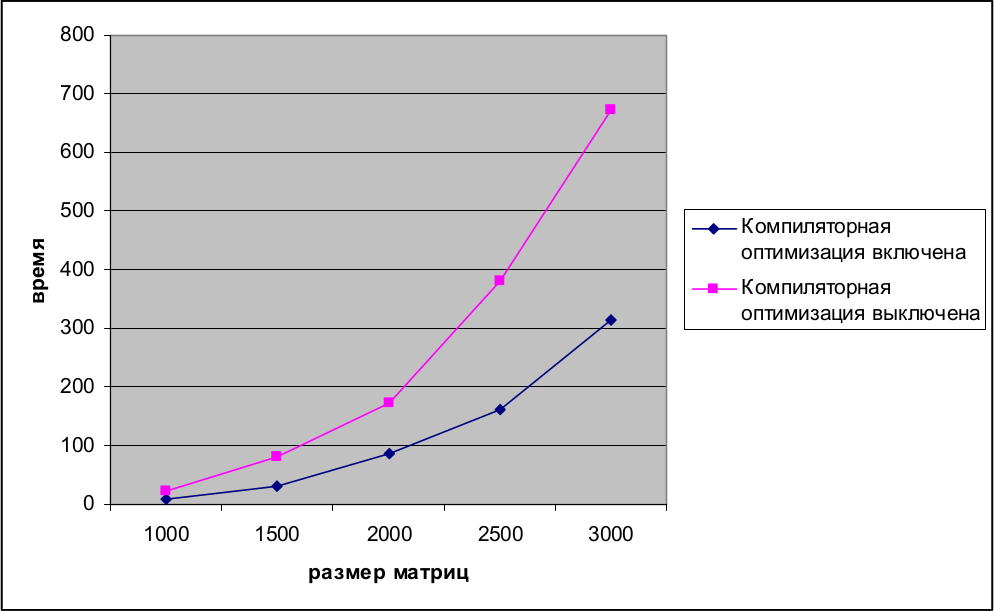
\includegraphics[scale=0.32]{res/pic004}
\caption{Графики зависимости времени выполнения оптимизированной и неоптимизированной версий последовательного алгоритма}
\end{figure}

\end{frame}

%------------------------------------------------
\subsection{Базовый параллельный алгоритм умножения матриц}
%------------------------------------------------

\begin{frame}
\frametitle{Базовый параллельный алгоритм умножения матриц}

Рассмотрим параллельный алгоритм умножения матриц, в основу которого будет положено разбиение
матрицы A на непрерывные последовательности строк (горизонтальные полосы).

\begin{figure}
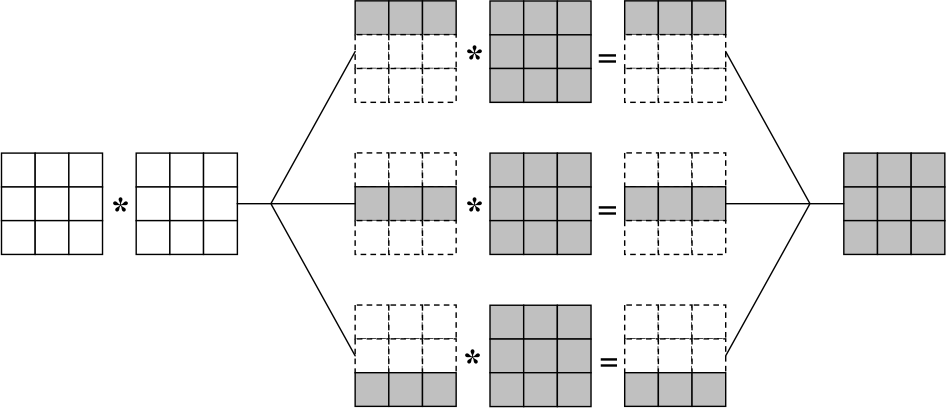
\includegraphics[scale=0.32]{res/pic005}
\caption{Организация вычислений при выполнении параллельного алгоритма умножения матриц, основанного на разделении матриц по строкам}
\end{figure}

\end{frame}

%------------------------------------------------

\begin{frame}
\frametitle{Базовый параллельный алгоритм умножения матриц}

Выделенные базовые подзадачи характеризуются одинаковой вычислительной трудоемкостью и равным объемом передаваемых данных. Если размер матриц $n$ оказывается больше, чем число вычислительных элементов (процессоров и/или ядер) $p$, базовые подзадачи можно укрупнить.\\~\\

Для вычисления одного элемента результирующей матрицы необходимо выполнить скалярное
умножение строки матрицы А на столбец матрицы В. Выполнение скалярного умножения включает $(2n-1)$
вычислительных операций. Каждый поток вычисляет элементы горизонтальной полосы результирующей
матрицы, число элементов в полосе составляет $n^2 /p$. Тогда общее время:

\begin{center}
$T_{\text{calc}} = \frac{n^2(2n-1)}{p} \times \tau$
\end{center}

\end{frame}

%------------------------------------------------

\begin{frame}
\frametitle{Базовый параллельный алгоритм умножения матриц}

Выделенные базовые подзадачи характеризуются одинаковой вычислительной трудоемкостью и равным объемом передаваемых данных. Если размер матриц $n$ оказывается больше, чем число вычислительных элементов (процессоров и/или ядер) $p$, базовые подзадачи можно укрупнить.\\~\\

Для вычисления одного элемента результирующей матрицы необходимо выполнить скалярное
умножение строки матрицы А на столбец матрицы В. Выполнение скалярного умножения включает $(2n-1)$
вычислительных операций. Каждый поток вычисляет элементы горизонтальной полосы результирующей
матрицы, число элементов в полосе составляет $n^2 /p$. Тогда общее время:

\begin{center}
$T_{\text{calc}} = \frac{n^2(2n-1)}{p} \times \tau$
\end{center}

\end{frame}

%------------------------------------------------

\begin{frame}
\frametitle{Базовый параллельный алгоритм умножения матриц}

Для того, чтобы разработать параллельную программу, реализующую описанный подход, при помощи технологии OpenMP, необходимо внести минимальные изменения в функцию умножения матриц.

\begin{figure}
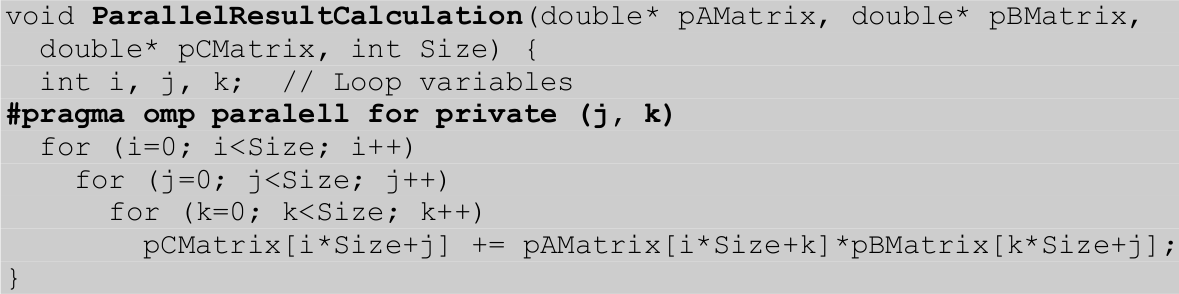
\includegraphics[scale=0.28]{res/pic006}
\caption{Базовый параллельный алгоритм умножения матриц}
\end{figure}

Данная функция производит умножение строк матрицы А на столбцы матрицы B с использованием нескольких параллельных потоков. Каждый поток выполняет вычисления над несколькими соседними строками матрицы A.

\end{frame}

%------------------------------------------------

\begin{frame}
\frametitle{Базовый параллельный алгоритм умножения матриц}

Результаты выполнения паралельного алгоритма:

\begin{figure}
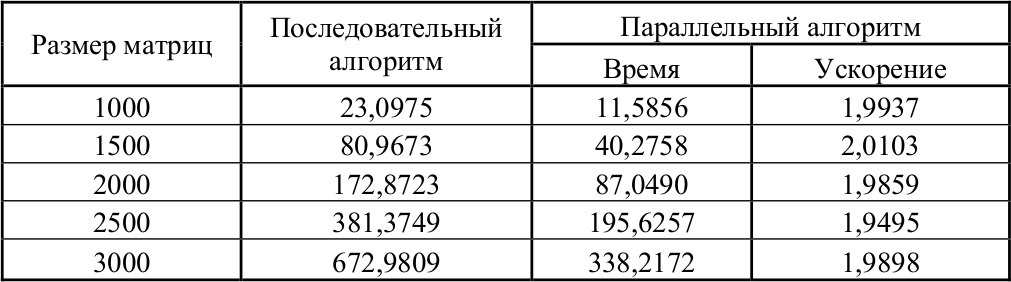
\includegraphics[scale=0.28]{res/pic007}
\caption{Результаты вычислительных экспериментов для параллельного алгоритма умножения
матриц при ленточной схеме разделении данных по строкам}
\end{figure}

\end{frame}


%------------------------------------------------
\subsection{Алгоритм, основанный на ленточном разделении данных}
%------------------------------------------------

\begin{frame}
\frametitle{Алгоритм, основанный на ленточном разделении данных}

В рассмотренном ранее алгоритме, только матрица A распределялась между параллельно выполняемыми потоками. Попробуем распаралелить и матрицу B.

\begin{figure}
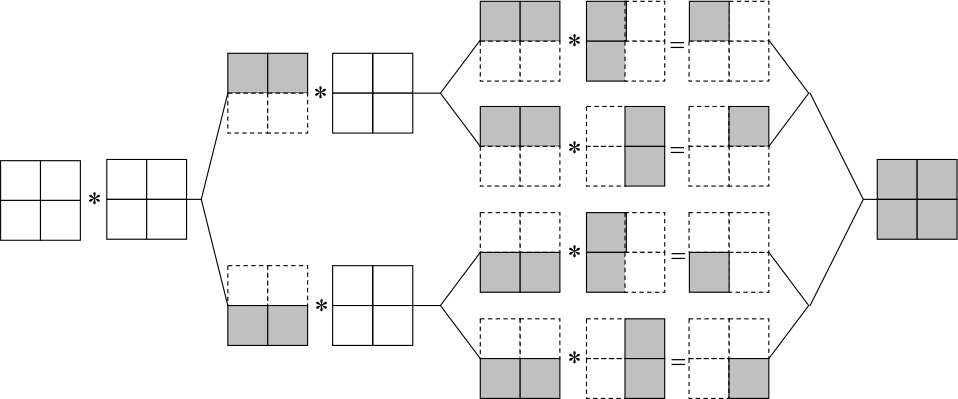
\includegraphics[scale=0.28]{res/pic008}
\caption{Организация параллельных вычислений при выполнении параллельного алгоритма умножения матриц, основанного на ленточном разделении данных, и использованием четырех потоков}
\end{figure}

\end{frame}

%------------------------------------------------

\begin{frame}
\frametitle{Алгоритм, основанный на ленточном разделении данных}

Для разделения матрицы A на горизонтальные полосы нужно разделить итерации внешнего цикла, а потом необходимо разделить итерации внутреннего цикла для разделения матрицы В на вертикальные полосы.

\begin{figure}
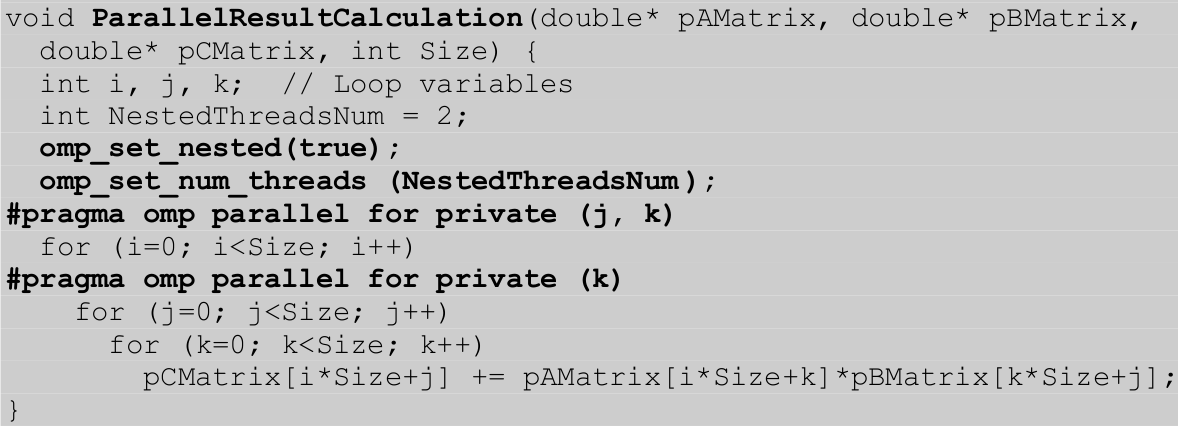
\includegraphics[scale=0.28]{res/pic009}
\caption{Алгоритм, основанный на ленточном разделении данных}
\end{figure}

\end{frame}

%------------------------------------------------

\begin{frame}
\frametitle{Алгоритм, основанный на ленточном разделении данных}

Вычислительные эксперименты для оценки эффективности параллельного алгоритма умножения матриц при ленточном разделении данных не показал выигрыша относительно базового параллельного алгоритма.

\begin{figure}
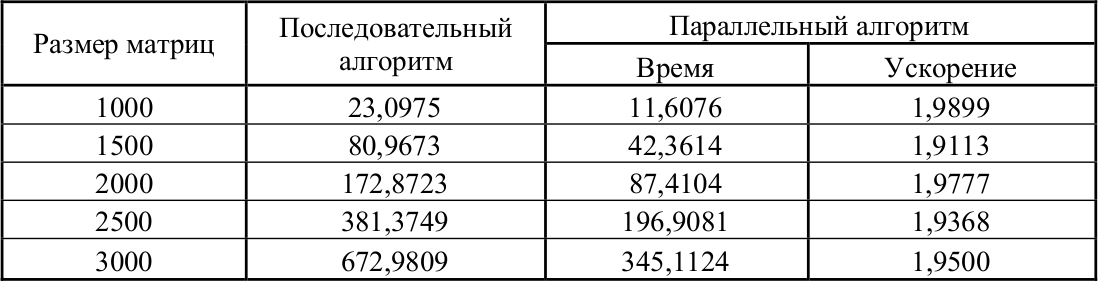
\includegraphics[scale=0.28]{res/pic010}
\caption{Результаты вычислительных экспериментов для параллельного алгоритма умножения матриц при ленточной схеме разделения данных}
\end{figure}

\end{frame}

%------------------------------------------------
\subsection{Блочный алгоритм умножения матриц}
%------------------------------------------------

\begin{frame}
\frametitle{Блочный алгоритм умножения матриц}

При построении параллельных способов выполнения матричного умножения наряду с рассмотрением матриц в виде наборов строк и столбцов широко используется блочное представление матриц.\\~\\

В этом подходе не только результирующая матрица, но и матрицы-аргументы матричного умножения разделяются между потоками параллельной программы на прямоугольные блоки. Такой подход позволяет добиться большей локализации данных и повысить эффективность использования кэш!
\end{frame}

%------------------------------------------------

\begin{frame}
\frametitle{Блочный алгоритм умножения матриц}

При построении параллельных способов выполнения матричного умножения наряду с рассмотрением матриц в виде наборов строк и столбцов широко используется блочное представление матриц.\\~\\

В этом подходе не только результирующая матрица, но и матрицы-аргументы матричного умножения разделяются между потоками параллельной программы на прямоугольные блоки. Такой подход позволяет добиться большей локализации данных и повысить эффективность использования кэш!\\~\\

К числу алгоритмов, реализующих описанный подход, относятся алгоритм Фокса (Fox) и алгоритм Кэннона (Cannon).
\end{frame}

%------------------------------------------------

\begin{frame}
\frametitle{Блочный алгоритм умножения матриц}
Будем предполагать, что все матрицы являются квадратными размера $n \times n$, количество блоков по горизонтали и вертикали являются одинаковым и равным $q$ (т.е. размер всех блоков равен $k \times k$, $k=\frac{n}{q}$).

\begin{figure}
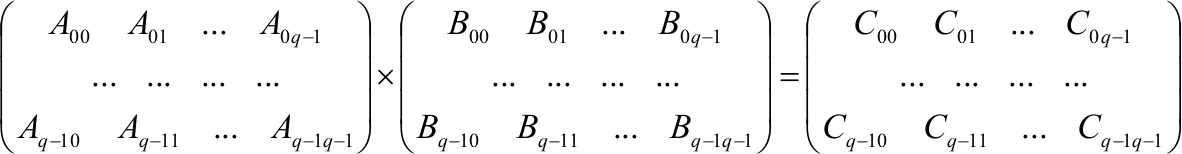
\includegraphics[scale=0.28]{res/pic011}
\caption{Представление данных операция матричного умножения матриц А и B в блочном виде}
\end{figure}

Тогда каждый блок $C_{i,j}$ матрицы $C$ определяется в соответствии с выражением:

\begin{center}
$C_{i,j} = \sum\limits^{q-1}_{s=0}(A_{i,s} \times B_{s,j})$
\end{center}

\end{frame}

%------------------------------------------------

\begin{frame}
\frametitle{Блочный алгоритм умножения матриц}
На каждой итерации $i$ алгоритма $i$-ый блок полосы матрицы $A$ умножается на $i$-ый блок полосы матрицы $B$, результат умножения блоков прибавляется к блоку результирующей матрицы.

\begin{figure}
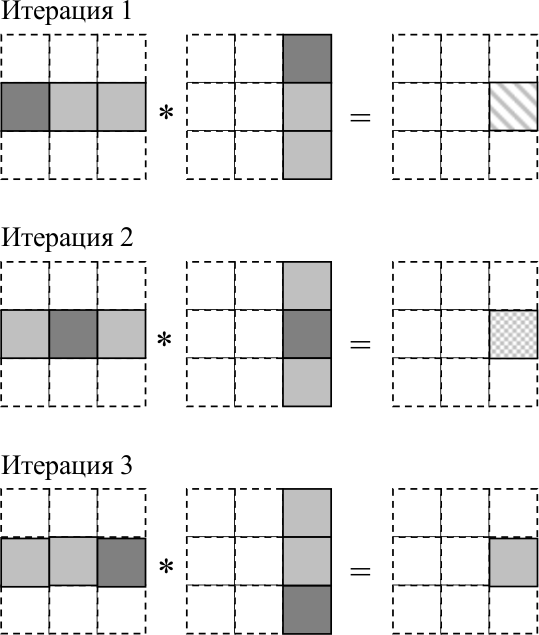
\includegraphics[scale=0.28]{res/pic012}
\caption{Представление данных операция матричного умножения матриц А и B в блочном виде}
\end{figure}

\end{frame}

%------------------------------------------------

\begin{frame}
\frametitle{Блочный алгоритм умножения матриц}
Каждый поток вычисляет элементы блока результирующей матрицы. Для этого каждый поток должен выполнить GridSize итераций алгоритма, каждая такая итерация есть умножение матричных блоков, итерации выполняются внешним циклом for по переменной iter.

\begin{figure}
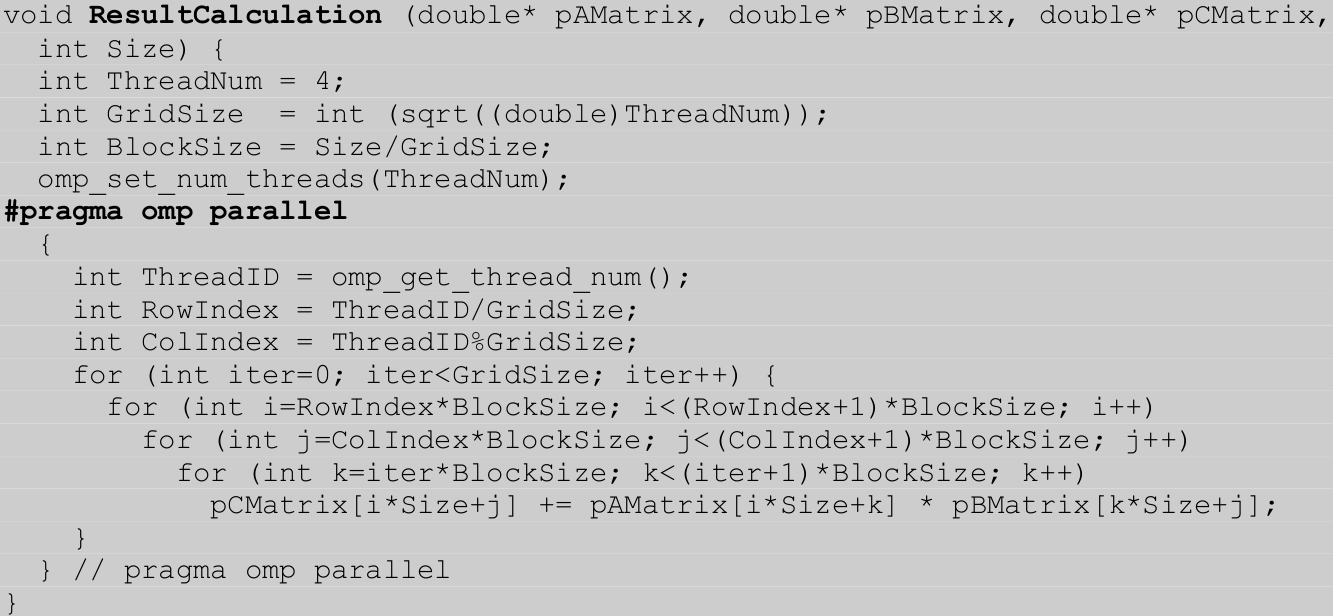
\includegraphics[scale=0.25]{res/pic013}
\caption{Блочный алгоритм умножения матриц}
\end{figure}

\end{frame}

%------------------------------------------------

\begin{frame}
\frametitle{Блочный алгоритм умножения матриц}

Результат очень близок к тому, что было получено ранее

\begin{figure}
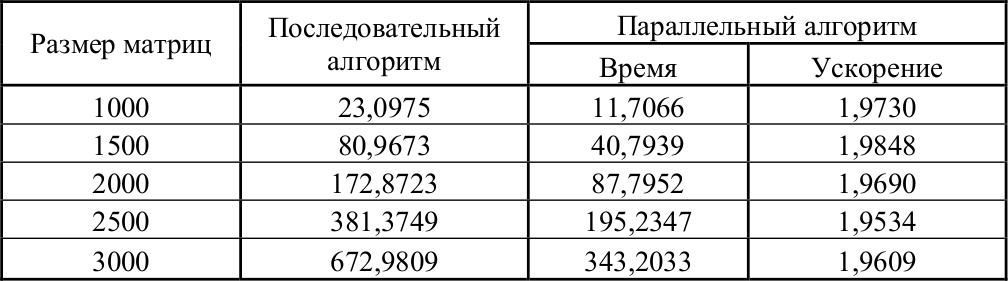
\includegraphics[scale=0.25]{res/pic014}
\caption{Результаты вычислительных экспериментов для параллельного блочного алгоритма умножения матриц}
\end{figure}

\end{frame}

%------------------------------------------------
\subsection{Кэш-эффективный блочный алгоритм}
%------------------------------------------------

\begin{frame}
\frametitle{Кэш-эффективный блочный алгоритм}

Значительная доля времени умножения матриц тратится на многократное чтение элементов матриц A и B из оперативной памяти в кэш!\\~\\

Для вычисления первого элемента строки результирующей матрицы необходимо прочитать в кэш все элементы первой строки матрицы А и первого столбца матрицы В, при этом, поскольку матрица В хранится в памяти построчно, то элементы одного столбца располагаются в оперативной памяти с некоторым интервалом. Таким образом, в кэш считывается не один столбец матрицы В, а сразу несколько столбцов.\\~\\

Реализуем разделение на блоки таким образом, чтобы размер блока был настолько мал, что три блока, участвующие в умножении на данной итерации, возможно было поместить в кэш.

\end{frame}

%------------------------------------------------

\begin{frame}
\frametitle{Кэш-эффективный блочный алгоритм}

Размер матричного блока равен 250. Это обеспечивает одновременное хранение трёх матричных блоков в в кэш объёмом 2 Мб.

\begin{figure}
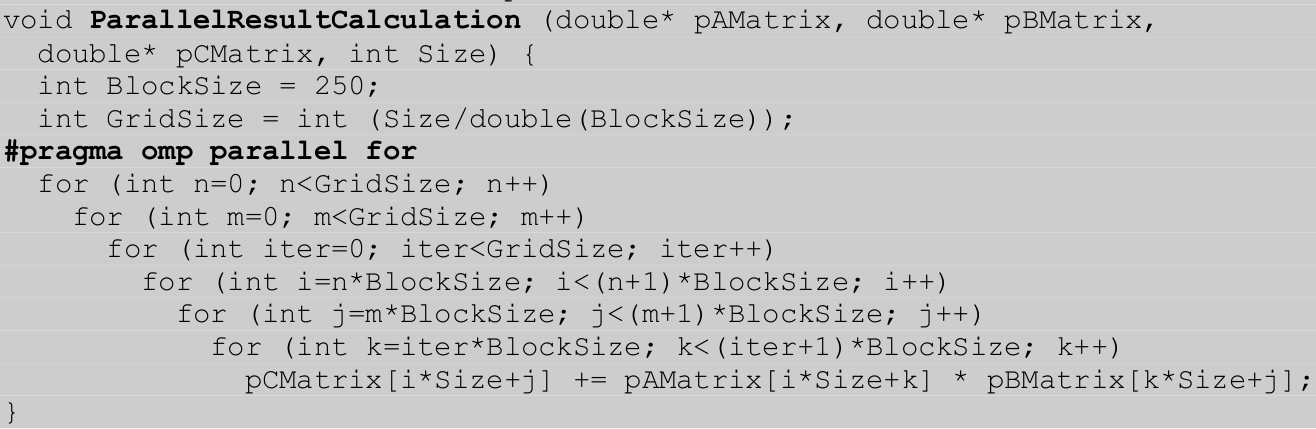
\includegraphics[scale=0.25]{res/pic015}
\caption{Результаты вычислительных экспериментов для параллельного блочного алгоритма умножения матриц}
\end{figure}

\end{frame}

%------------------------------------------------

\begin{frame}
\frametitle{Кэш-эффективный блочный алгоритм}

Размера матричного блока (параметр k) оказывает существенное влияние на на эффективность параллельного алгоритма.

\begin{figure}
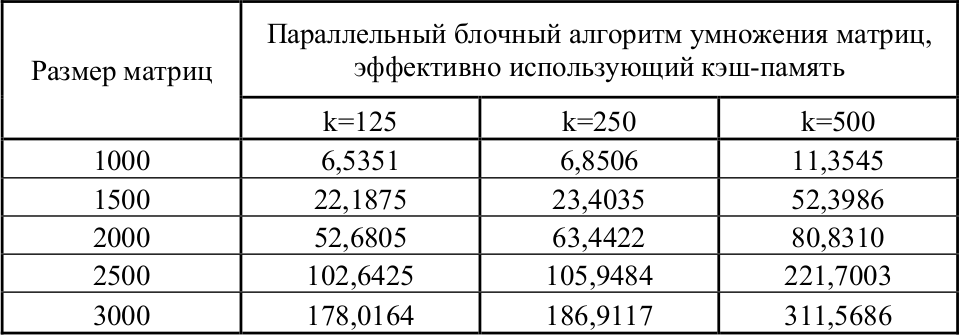
\includegraphics[scale=0.30]{res/pic016}
\caption{Время выполнения параллельного блочного алгоритма умножения матриц при разных
размерах матричных блоков}
\end{figure}

\end{frame}

%------------------------------------------------

\begin{frame}
\frametitle{Кэш-эффективный блочный алгоритм}

\begin{figure}
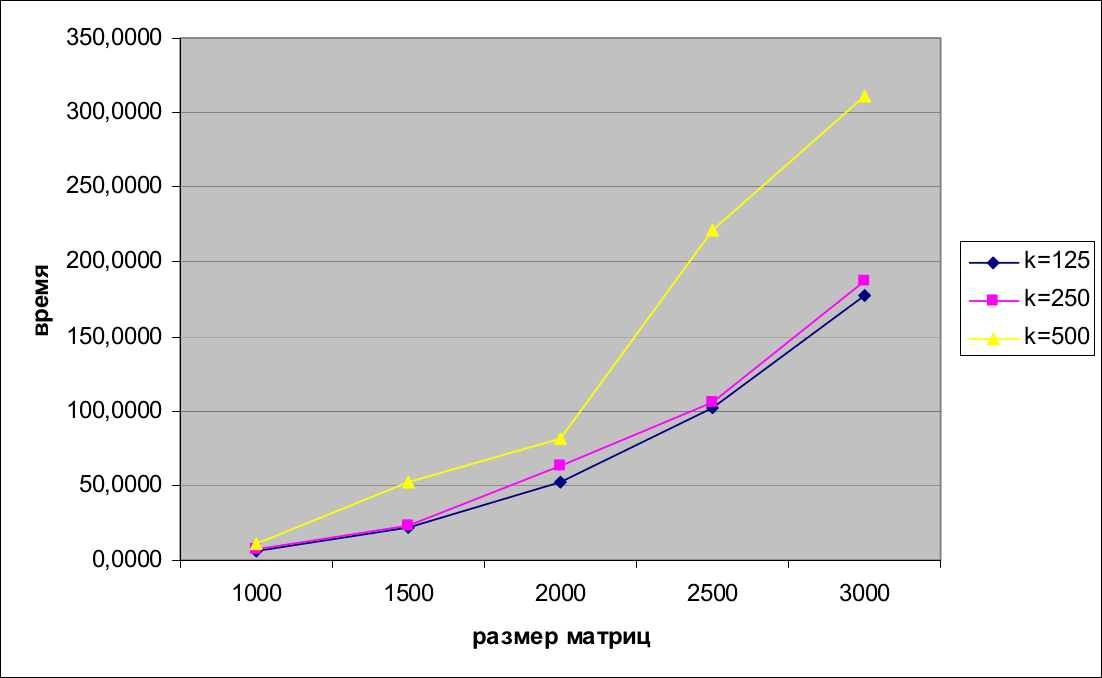
\includegraphics[scale=0.27]{res/pic017}
\caption{Время выполнения параллельного алгоритма умножения матриц, ориентированного на эффективное использование кэш-памяти, при разных размерах матричных блоков}
\end{figure}

\end{frame}

%------------------------------------------------
\section{Заключение}
%------------------------------------------------

\begin{frame}
\frametitle{Заключение}

\begin{figure}
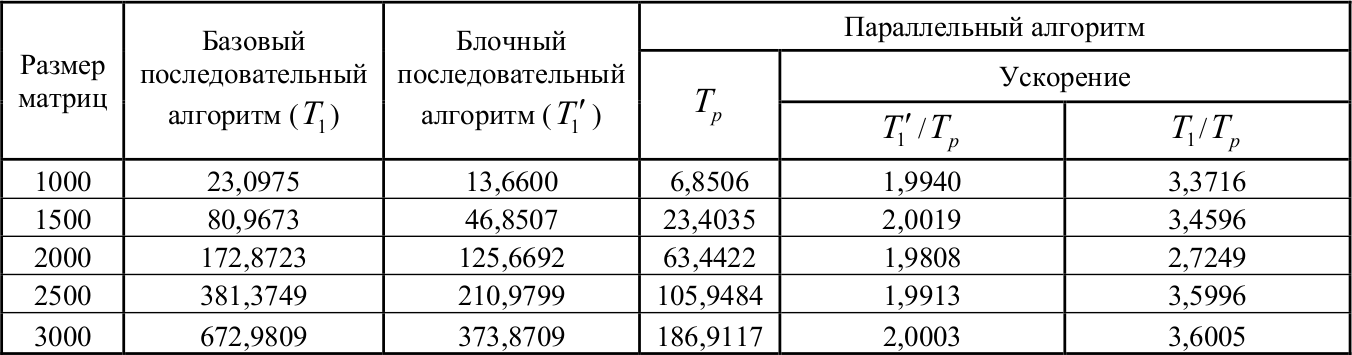
\includegraphics[scale=0.25]{res/pic018}
\caption{Результаты вычислительных экспериментов для параллельного блочного алгоритма умножения матриц, ориентированного на эффективное использование кэш-памяти}
\end{figure}

\end{frame}

%------------------------------------------------

\begin{frame}
\frametitle{Заключение}

\begin{figure}
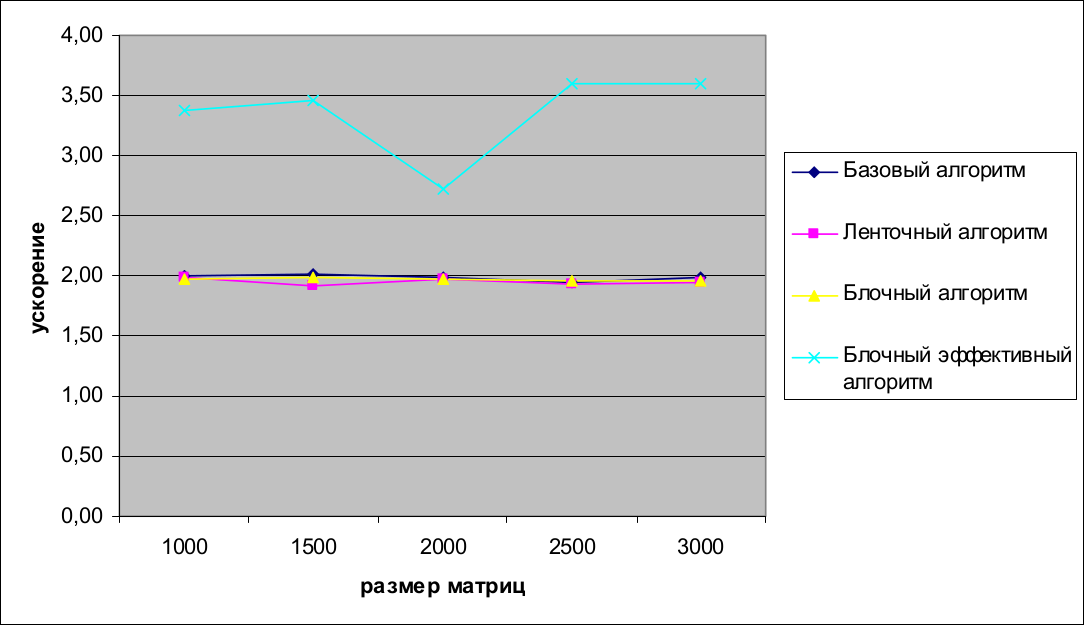
\includegraphics[scale=0.30]{res/pic019}
\caption{Сводный график всех рассмотренных алгоритмов}
\end{figure}

\end{frame}

%------------------------------------------------
\section{Источники}
%------------------------------------------------

\begin{frame}
\frametitle{Источники}
\footnotesize{
\begin{thebibliography}{99} % Beamer does not support BibTeX so references must be inserted manually as below
\bibitem[Kolton, 2013]{p1} Колтон С.Л., Хозяинов И.А.
\newblock Кэш-независимые алгоритмы
\newblock \emph{Санкт-Петербургский государственный политехнический университет, Институт информационных технологий и управления, Кафедра компьютерных систем и программных технологий} -- реферат по дисциплине Вычислительные системы, СПб, 2013.
\end{thebibliography}

\begin{thebibliography}{98}
\bibitem[Labutina, 2007]{p1} Лабутина А.А.
\newblock Параллельные методы матричного умножения
\newblock \emph{Нижегородский государственный университет им. Н.И.Лобачевского} -- материалы учебного курса Введение в методы параллельного программирования, Нижний Новгород, 2007.
\end{thebibliography}

\begin{thebibliography}{97}
\bibitem[Frigo, 2015]{p1} Matteo Frigo, Charles E. Leiserson, Harald Prokop, Sridhar Ramachandran
\newblock Cache-Oblivious Algorithms
\newblock \emph{MIT Laboratory for Computer Science, 545 Technology Square, Cambridge, MA 02139}.
\end{thebibliography}
}
\end{frame}


%------------------------------------------------
\section{Вопросы}
%------------------------------------------------

\begin{frame}
\Huge{\centerline{Вопросы?}}
\end{frame}

%----------------------------------------------------------------------------------------

\end{document}